\begin{frame}
    \titlepage
\end{frame}

\begin{frame}
    \frametitle{Context \& Motivation}
    \centering
    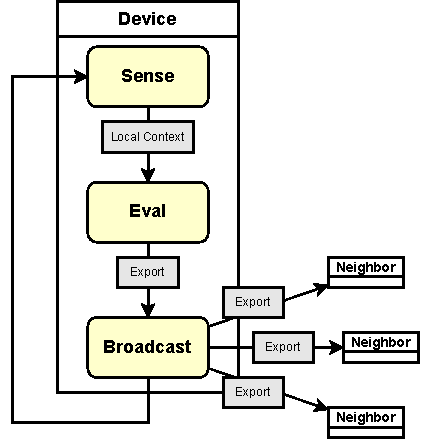
\includegraphics[height=5cm]{figures/proactive-model.pdf}
    \begin{blockitems}{Distributed systems, with these characteristics}
        \item \textbf{openness}: a constantly and unexpectedly changing environment
        \item \textbf{large scale}: huge number of heterogeneous devices
        \item \textbf{intrinsic adaptiveness}: need for overall system resilience
    \end{blockitems}
\end{frame}

\begin{frame}
    \frametitle{The goal of this thesis}
    \begin{blockitems}{Desiderata}
        \item declaratively describe the behavior of distributed systems
        \item coordination through \textbf{self-organization}
        \item fine-tune the \textbf{dynamics} and the \textbf{timing} of computations
    \end{blockitems}
    \begin{blockitems}{Goal}
        \item use FRP to express programs as reactions to changes in the environment
        \item ultimate vision: \textbf{Functional Reactive Self-Organization}
    \end{blockitems}
\end{frame}

\begin{frame}
    \frametitle{Background}
    \begin{blockitems}{Aggregate Computing}
        \item programming \textbf{aggregates} of devices instead of individual ones
        \item programs expressed as \textbf{computational fields} and their \textbf{functional composition}
        \item computed by a network of devices sharing messages with each other
        \item strong \textbf{decentralization}
        \item based on a formal \textbf{field calculus}
    \end{blockitems}
    \begin{blockitems}{Functional Reactive Programming (FRP)}
        \item paradigm shift over the \textit{observer pattern}
        \item built around the notion of (automatic) \textbf{propagation of change}
        \item declaratively construct a \textbf{dependency graph} of \textit{cells} and \textit{streams} and let the FRP engine propagate changes
        \item strong focus on the \textbf{compositionality} aspect
    \end{blockitems}
\end{frame}

\begin{frame}
    \frametitle{Proactive model of the Field Calculus}
    \begin{columns}
        \begin{column}{0.4\textwidth}
            Computation is split into \textbf{rounds} that are repeatedly executed by each device:
            \begin{itemize}
                \item \textbf{sense}: gather information from the environment and construct a \textit{local context}
                \item \textbf{eval}: evaluate the aggregate program against the local context, producing an \textit{export}
                \item \textbf{broadcast}: send the export to all neighbors
            \end{itemize}
        \end{column}
        \begin{column}{0.6\textwidth}
            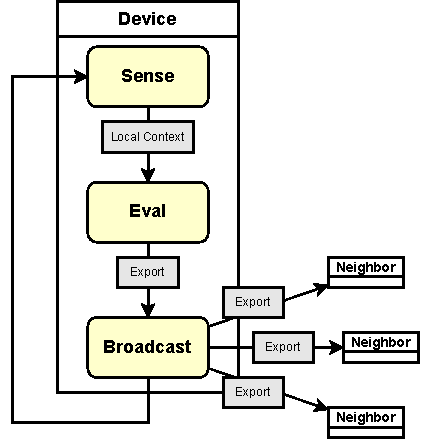
\includegraphics[width=\textwidth]{figures/proactive-model.pdf}
        \end{column}
    \end{columns}
\end{frame}

\begin{frame}
    \frametitle{Shortcomings of the proactive model}
    \begin{blockitems}{Wasteful computation}
        \item computation happens regardless of the existence of significant changes in the environment
        \item no native way to express \textit{reactions} to changes in the environment
        \item sub-computations that are not affected by changes in the environment need to be re-evaluated at each round
    \end{blockitems}
    \begin{blockitems}{Wasteful message exchange}
        \item exports are broadcast even if they didn't change significantly since the last round
        \item localized changes in the environment needlessly affect the entire network
    \end{blockitems}
\end{frame}

\begin{frame}
    \frametitle{Introducing a reactive model}
    \begin{blockitems}{A reactive context}
        \item an abstraction over the environment from the POV of a single device
        \item provides \textbf{sensors} and \textbf{neighborhood} information in a \textit{reactive} way (thanks to \textit{cells} from FRP)
    \end{blockitems}
    \begin{blockitems}{Expressing aggregate computations as \textit{flows}}
        \item \textbf{Flow} = a \textit{reactive} representation of a field evolving over time
        \item encapsulates a way to produce a \textit{cell} of its \textit{exports} from the \textit{context} on which it is run
        \item an entire aggregate program can be represented as a flow and run on each device's context
    \end{blockitems}
\end{frame}

\begin{frame}
    \frametitle{}
    \begin{blockitems}{Differences from the proactive model}
        \item no longer based on \textit{computation rounds}
        \item computations happen as soon as events of interest are recognized (and only in those occasions)
        \item exports are broadcast only after a significant change
    \end{blockitems}

\end{frame}

\begin{frame}
    \frametitle{Demo: Gradient with Obstacles}
\end{frame}

\begin{frame}
    \frametitle{Conclusions \& Future Work}
\end{frame}
